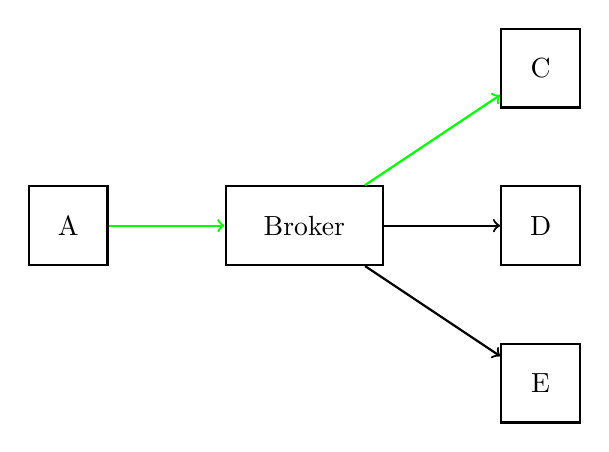
\begin{tikzpicture}[thick]

  % Rectangles

  \begin{scope}
    \node(A) [draw,rectangle,minimum width=1cm,minimum height=1cm]{A};
  \end{scope}

  \begin{scope}[xshift=3cm]
    \node(Broker) [draw,rectangle,minimum width=2cm,minimum height=1cm]{Broker};
  \end{scope}

  \begin{scope}[xshift=6cm, yshift=2cm]
    \node(C) [draw,rectangle,minimum width=1cm,minimum height=1cm]{C};
  \end{scope}

  \begin{scope}[xshift=6cm]
    \node(D) [draw,rectangle,minimum width=1cm,minimum height=1cm]{D};
  \end{scope}

  \begin{scope}[xshift=6cm, yshift=-2cm]
    \node(E) [draw,rectangle,minimum width=1cm,minimum height=1cm]{E};
  \end{scope}

  % Arrows

  \draw[green, ->](A) edge (Broker);

  \draw[green,->] (Broker) edge (C);

  \draw[->]     (Broker) edge (D)
                (Broker) edge (E);
\end{tikzpicture}
